% CHAPTER 1
\chapter{EVALUATION OF FAST INERTIAL RESPONSE AND SYNTHETIC INERTIA IMPLEMENTATION}
\label{chp:6}
Increase in share of renewable energy in the installed capacity brought operational problems. Due to the fact that PV systems do not have rotational mass at all or wind turbines with full-scale or partial scale power electronics do not effectively contribute the grid aggregated inertia, the power system with increasing renewable energy penetration will be exposed to high RoCoF for the frequency disturbances. This implies that system will encounter unacceptable RoCoF values (around the RoCoF protection settings of the generating units) in the normal operation as long as the renewable penetration continues. Therefore, the upcoming future power system will require auxiliary services such as synthetic i.e. virtual inertial support from all generation technologies that includes power electronics. \par
Renewable energy systems produces power according to the type of its power source. The input power is constant for an instant since the source (solar radiation, wind speed etc.) is constant. Therefore, the operation of renewable systems is different from the conventional power plants in which input power can be controlled by the operator. Nonetheless, an additional energy source is required in the renewable systems in order to increase active power as desired. For this purpose, rotational kinetic energy in wind turbine blades and generator can be utilized. In this way, the wind turbines are able to increase their active output power by extracting the kinetic energy stored in the turbine equivalent inertia. However, the amount of active power increase can be either constant as in the case of Chapter \ref{chp:4} or dynamic (proportional to RoCoF) as in the case of Chapter \ref{chp:5}.
\section{Fast Inertial Support}
Wind turbines with full-scale power electronics can adjust its active power by controlling its output torque. Therefore, the active power can be quickly raised by extracting the stored energy in the turbine inertia. However, the maximum value of the active power that can be extracted depends on the operating conditions. Since the generator active power is also dependent on its speed, turbine power cannot be increased up to rated power but to half of the rated power in wind speeds lower than 5m/s. In wind speeds higher than 10m/s, the active power before the support is already close to its rated value. Therefore, the increase in the active power is limited as 10\% (as long as converter rating has the capacity) in high wind scenarios. \par
In this study, the wind turbine can increase its active output power by 1.2MW in the wind speeds between 5m/s and 8m/s for fast inertial response. The highest active power release is found in the wind speed 6.5m/s as 1.3MW. Besides, wind turbines can contribute better in low wind scenarios than that of high wind speed for short time intervals. However, when the active power increase is limited with 10\%, \par
It should be noted that the frequency disturbance occurs due to the unbalance between input mechanical power and output powers of the generators. Hence, the additional amount of active power that is provided from renewable energy sources in such instants is favourable. This is why the amount of increase in the active power is important. Therefore, knowledge of active power limits reveals the potential of wind turbines with FSPC in order to contribute the frequency stability of the power systems.\par
Fast inertial response can be provided within different time durations up to 30 seconds. Since the larger amount of support might result in higher speed deviations, the support time might be decreased. In contrary, higher support durations can be achieved with lower amount of fast inertial response. Notice that turbine will decrease its output power after the support period to restore its speed. Therefore, the additional energy will be the zero at the end of the support. \par
Fast inertial response in this study is not a direct function of the RoCoF. In other words, the support power is independent from RoCoF or frequency deviation. However, the activation of the support is based on a RoCoF threshold of 0.1Hz/s with the frequency dead-band 10mHz. A RoCoF indexing can be developed to obtain different support power values. In this case, the indexing scheme requires a RoCoF threshold and different RoCoF intervals. The highest RoCoF interval corresponds to the most severe frequency disturbances case (RoCoF above 0.5Hz/s) and requires the highest amount of fast inertial support release with highest available support time. Meanwhile, the lowest RoCoF interval would be assigned to lowest inertial support release with time duration in order not to result higher speed deviation. It should be noted that the higher energy extraction might even result in the stall of the turbine. Nonetheless, critical instant following the disturbance is much more important than the turbine speed recovery. Hence, grid operators might choose to extract the available active power in the expense of turbine stall according to the optimized decision.
\section{Synthetic Inertia Implementation}
Even though wind turbine power can be increased as desired between 0.1pu and 0.45pu range by using fast inertial support, the fastest release of the power independent of the frequency is not the best solution especially for weak power grids. Although additional amount of power is released in the disturbances, restoration of the energy to wind turbine might cause a second frequency decrease in the grid. Therefore, the increase amount should be in coordination with the grid frequency behavior. This is why dynamic frequency response is obtained with the synthetic inertia implementation in the Chapter \ref{chp:5}. \par
By adjusting active power according to the RoCoF of the grid, the active power is increased or decreased depending on the grid status. If the frequency decreases, additional amount of active power proportional to RoCoF will be injected to grid. The advantage of the dynamic frequency response is the fact that the active power is decreased below the pre-disturbance power value as grid RoCoF is positive. This implies that the restoration of the turbine speed begins with positive RoCoF avoiding a second drop in the frequency.\par
In order to observe the effects of synthetic inertia implementation, a dynamical 9-bus test system is constructed in Matlab-Simulink environment. The test system is composed of the conventional generators and subjected to a frequency disturbance with a load connection. In order to see the effects of the renewable energy penetration, a wind farm with 20 turbines is connected to system. In the 10\% Renewable Case, the system frequency behavior is not affected from the renewable penetration. The maximum RoCoF of 0.23Hz/s is observed in the system. The maximum RoCoF decreased down to 0.25Hz/s in the Reduced Inertia Case. The frequency behavior is improved by the synthetic inertia by lowering the RoCoF values down to 0.19Hz/s in 10\% Renewable Case and 0.21Hz/s in the Reduced Inertia Case.
\par
The most important feature of the synthetic inertia implementation is the RoCoF dependency. The inertial support in this method does decrease the active power as soon as RoCoF turns positive meaning that turbine speed recovery can be started. Thus, the speed recovery of the synthetic inertia method begins when the frequency nadir is reached.\par
The synthetic inertia implementation is used for improving the transient behavior of the frequency. In the literature, variety of inertia constants are emulated in variable speed wind turbines between the inertia constant up to 10 seconds \cite{Gonzalez-Longatt2013},\cite{Gonzalez-Longatt}. Chapter \ref{chp:4} demonstrates that the wind turbines are able to increase its active power temporarily by 0.45pu. In this study inertia constants more than 10 seconds are also tested. Nonetheless, the inertia constants more than 10s is not possible in the high wind speed range. Nonetheless, inertia constant of 10s is applicable for whole speed range. Inertia constants above 10s can also be achievable as long as the converter rating is available. In the worst case scenario, output power saturates to the limit for a part of the support duration. However, as the RoCoF decreases, output power can follow the commanded output power.\par 
Synthetic inertia implementation in the Turkish electricity network is also evaluated based on the hourly generation data from 2018. The effect of the varying generation profile is calculated by considering wind and solar energy. It is shown that the decrease in the aggregated inertia constant of the grid can be compensated with the help of synthetic inertia implementation to wind turbines with FSPC. In fact, the wind turbines with FSPC are able to compensate not only the decrease due to their existing structure but also the decrease due to other wind turbines (DFIG and Type I-II) and PV systems. This is why the synthetic inertia should be implemented in all of the wind turbines with full-scale power converter.
\section{Economical Motivations for Energy Providers}
As explained in Section \ref{section-price}, renewable energy systems in Turkey and most of the EU countries sell electricity with feed-in tariff. It basically means that all the generated energy is sold without trading in day-ahead market. Even though the problems are arising with renewable energy systems, the energy providers would not be a volunteer for ancillary services unless the regulations impose sanctions or additional payment is provided to turbine owners. Hence, the system operator should prepare more advantageous compensation mechanisms in order to convince energy providers to implement grid supporting methods. \par
The system operators has already started preparing new frequency regulations. One of the examples is the Firm Frequency Response (FFR) by National Grid \cite{NationalGridElectricityTransmission2016}. FFR is basically frequency support method that is activated with the frequency thresholds. As the frequency falls below a pre-determined value, a response is required by the energy providers (either from synchronous generators or energy storage units). These energy providers are taken into operation according to their bids. The response is either non-dynamic (independent from the frequency shift) or dynamic (pre-determined percentage increased according to frequency). Moreover, the support power should be sustained up to 30 seconds dynamic response and up to 30 minutes for non-dynamic response for the primary \cite{Smethurst2017}. This is why the response is provided by synchronous generators and energy storage systems in which active power output can be adjusted as desired. It should be noted that this mechanism is not appropriate for the renewable energy systems where the output power can be increased up to 30 seconds by utilizing the stored energy in the inertia or DC-link capacitor.\par
Another frequency regulating mechanism is applied in USA according to the FERC 755 regulation \cite{FederalEnergyRegulatoryCommission2011}. The frequency regulation includes different metrics for payment such as capacity, performance and mileage. Based on this regulation, energy price for the high performance frequency regulation resources is increased over three times of the old price of the PJM which is a regional transmission company \cite{NECEnergySolutions2014}. Since one of the metrics effecting the payment is performance, the regulation is advantageous for energy storage systems that can adjust its active power quickly thanks to their power electronics interface.\par
When the wind turbine is used for inertial support mechanisms, additional power up to 0.45pu can be achieved for 3s or 0.1pu power with unlimited duration (as long as converter can handle). The longer time durations might cause problems for power converter such as heating. Even though the turbine injects significant amount of power to grid, the additional amount of energy (4000kWs) is negligible compared to daily energy production. Therefore, the payment for the additional amount of energy would not be beneficial to energy provider. \par
In order to investigate the economical side of the frequency regulating mechanisms in the renewable energy systems, a frequency support case is evaluated with two hypothetical payment methods. One of the methods takes into account of the additional energy supplied during the frequency disturbance. Other payment method considers the availability of the wind turbine. Table \ref{new_price} shows the average energy generation according to the measurements from site as well as the hypothetical profits from inertial support based on either additional energy or incentive. It is obvious that the wind turbine in this study produces electrical energy worth \$1679 each day in average. If the additional energy is sold with 248.2\$/MWh price (3.4xFeed-In Tariff), \$2.76 additional profit is yielded by assuming 10 daily support. This corresponds to 0.16\% of the daily profit and it is insignificant to energy provider. \par
\begin{table}[h!]
	\centering
	\begin{tabular}{ccc}
		\hline
		\multicolumn{3}{c}{Base Case Profit} \\
		Daily Energy Production & 23 & MWh \\
		Feed-In Tariff & 73 & \$/MWh \\
		Daily Generation & 1679 & \$ \\ \hline
		\multicolumn{3}{c}{Profit by Additional Energy} \\
		Energy From Single Support & 4000 & kWs \\
		\begin{tabular}[c]{@{}c@{}}Supported Energy Price\\ (3.4xFeed-In Tariff)\end{tabular} & 248.2 & \$/MWh \\
		Additional Profit for Single Support & \multicolumn{1}{l}{0.276} & \$ \\
		Number of Support (Daily) & \multicolumn{1}{l}{10} & \multicolumn{1}{l}{} \\
		Additional Profit & 2.76 & \$ \\ \hline
		\multicolumn{3}{c}{Profit with Incentive} \\
		Daily Energy Production& 23 & MWh \\
		Supported Feed-In Tariff & 79 & \$/MWh \\
		Additional Profit & 138 & \$ \\ \hline
	\end{tabular}
	\caption{Comparison of the Hypothetical Frequency Support Pricing Methods}
	\label{new_price}
\end{table}
Following an inertial support period, turbine will deliver lower power in order to restore its speed. Consequently, the energy injected by the turbine will be the same. Besides, the detection of the support energy is complicated for the system operator. It is not possible to distinguish the cases where the turbine injects inertial support or the wind speed increases in the site. Therefore, the grid operator cannot estimate a price from the additional energy concept.\par
\newpage
Second payment method is based on the availability of the wind turbine for the frequency regulation mechanisms. Notice that renewable energy systems get additional payment from the local content bonus. A similar incentive can be assigned to wind turbines for their availability for grid supporting mechanisms. For this purpose, the lowest local content bonus amount which is additional 0.6\cent/kWh for local turbine tower is used for this study. Therefore, the turbines providing synthetic inertia support is paid with 79\$/MWh. In this way, \$138 additional profit can be obtained regardless of the number of support or the additional energy. In this case, the energy provider can increase the average income by 8.2\%. Therefore, assigning incentives for the grid supporting services might be attractive for the energy providers. Moreover, system operators of the weak power grids might lean towards the inertial support by wind turbine operators even at the expense of the additional incentives to the energy providers.\par 
\begin{figure}[h!]
	\centering
	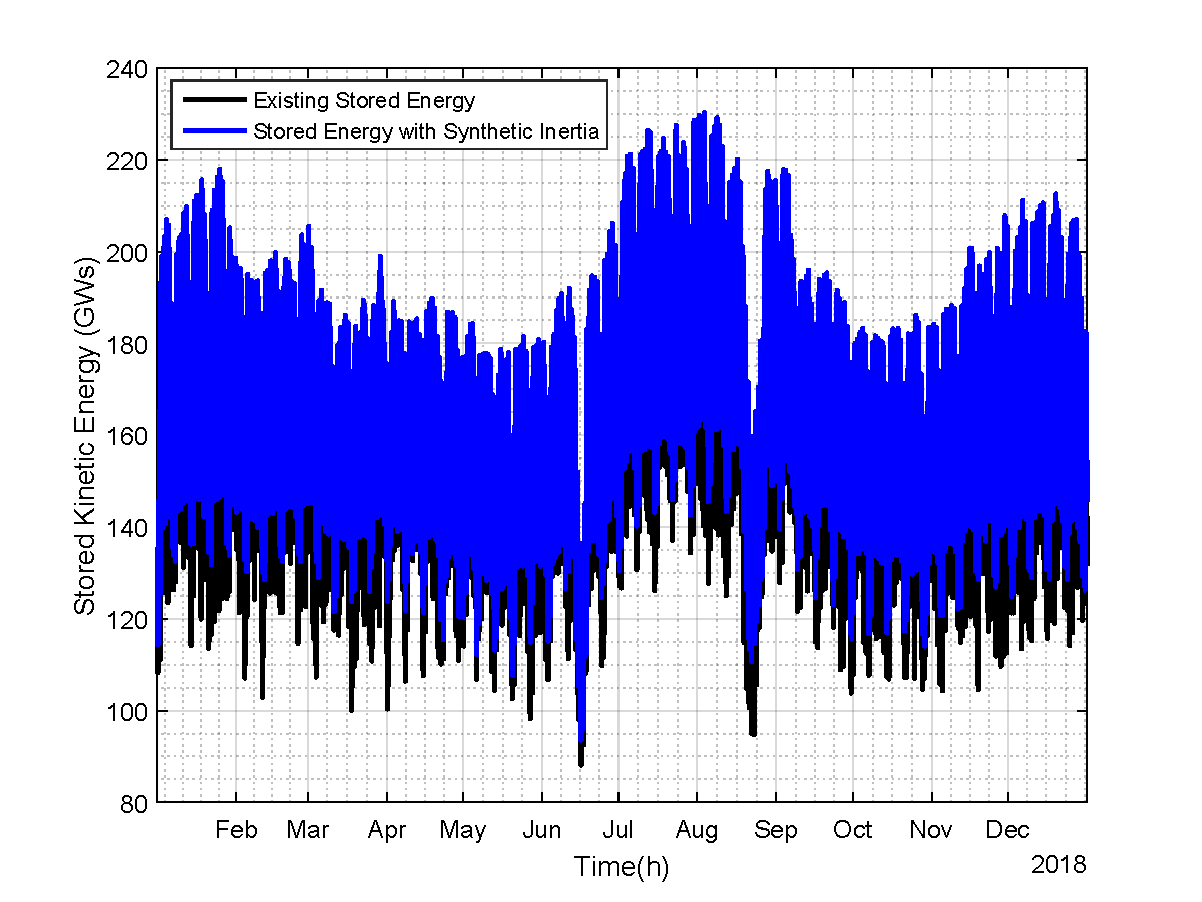
\includegraphics[width=0.95\linewidth]{storedenergyy.pdf}
	\caption{Variation of the Stored Kinetic Energy between 01 Jan. 2018 and 31 Dec. 2018 (hourly basis)}
	\label{gridstored}
\end{figure}
\newpage
The effect of the wind and solar energy is investigated at the end of Chapter \ref{chp:5}. It is shown that grid aggregated inertia constant depends on the wind and solar production. The variation of the kinetic energy stored in the grid is given in Fig. \ref{gridstored}. The average stored energy in the grid can be increased by 8\% with the synthetic inertia implementation. Notice that the difference between the existing stored energy and the one with synthetic inertia implementation is dependent on the share of wind and solar systems. Therefore, the difference between these energies will increase with the increasing renewable penetration. Therefore, the system operator should prepare frequency regulating regulations for the renewable energy systems. Moreover, a convincing solution should be constructed to avoid upcoming frequency stability problems. 
\newpage
\section{Conclusion}
This chapter compares two inertial support methods namely; fast inertial support and synthetic inertia methods. It is stated that fast inertial support can provide increased active power that is independent from the grid RoCoF. Even though grid RoCoF is improved as long as support is sustained, a secondary frequency dip might be encountered when the support is terminated. Therefore, fast inertial support might deteriorate the frequency stability of the weak power systems. On the contrary, synthetic inertia method adjust the active power according to the grid RoCoF. Therefore, the additional active power of the wind turbine is not ceased instantaneously but changed in a smoother way due to the fact that it is proportional to grid RoCoF.\par
Economical feasibility of the inertial support of wind turbines are also studied in this chapter. It is shown that inertial support payment based on the additional energy during frequency disturbances is not a convincing solution for the energy providers. Instead, energy provider can make additional profit with the inertial support implementation as long as they are paid with additional incentives. It should be noted that the new wind power plants that will be commissioned after 2020 will not benefit from feed-in tariff and local bonus content in Turkey. Therefore, a new incentive mechanism might be constructed with grid supporting services like wind turbine inertial support which will convince the energy providers. In this way, the reduction in grid effective inertia might be avoided and frequency stability of electricity grid is preserved.